\documentclass[12pt,a4paper]{exam}
\usepackage[utf8]{inputenc}
\usepackage[T1]{fontenc}
\usepackage{amsmath}
\usepackage{amsfonts}
%\usepackage{amssymb}
\usepackage{graphicx}
\usepackage{geometry}
\usepackage{enumitem}

\geometry{a4paper, margin=2cm}

\usepackage{cprotect}

\usepackage{xcolor}
\definecolor{maroon}{cmyk}{0, 0.87, 0.68, 0.32}
\definecolor{halfgray}{gray}{0.55}
\definecolor{ipython-frame}{RGB}{207, 207, 207}
\definecolor{ipython-bg}{RGB}{247, 247, 247}
\definecolor{ipython-red}{RGB}{186, 33, 33}
\definecolor{ipython-green}{RGB}{0, 128, 0}
\definecolor{ipython-cyan}{RGB}{64, 128, 128}
\definecolor{ipython-purple}{RGB}{170, 34, 255}
\usepackage{listings}
\lstdefinelanguage{iPython}{
	morekeywords={access,and,del,except,exec,in,is,lambda,not,or,raise},
	morekeywords=[2]{for,print,abs,all,any,basestring,bin,bool,bytearray,callable,chr,classmethod,cmp,compile,complex,delattr,dict,dir,divmod,enumerate,eval,execfile,file,filter,float,format,frozenset,getattr,globals,hasattr,hash,help,hex,id,input,int,isinstance,issubclass,iter,len,list,locals,long,map,max,memoryview,min,next,object,oct,open,ord,pow,property,range,reduce,reload,repr,reversed,round,set,setattr,slice,sorted,staticmethod,str,sum,super,tuple,type,unichr,unicode,vars,xrange,zip,apply,buffer,coerce,intern,elif,else,if,continue,break,while,class,def,return,try,except,import,finally,try,except,from,global,pass, True, False},
	sensitive=true,
	morecomment=[l]\#,%
	morestring=[b]',%
	morestring=[b]",%
	moredelim=**[is][\color{black}]{@@}{@@},
	%%
	%morestring=[s]{'''}{'''},% used for documentation text (mulitiline strings)
	%morestring=[s]{"""}{"""},% added by Philipp Matthias Hahn
	%%
	%morestring=[s]{r'}{'},% `raw' strings
	%morestring=[s]{r"}{"},%
	%morestring=[s]{r'''}{'''},%
	%morestring=[s]{r"""}{"""},%
	%morestring=[s]{u'}{'},% unicode strings
	%morestring=[s]{u"}{"},%
	%morestring=[s]{u'''}{'''},%
	%morestring=[s]{u"""}{"""}%
	%
	% {replace}{replacement}{lenght of replace}
	% *{-}{-}{1} will not replace in comments and so on
	%literate=
	%{\%}{{{\color{ipython-purple}+}}}1,
	%{á}{{\'a}}1 {é}{{\'e}}1 {í}{{\'i}}1 {ó}{{\'o}}1 {ú}{{\'u}}1,
	%{Á}{{\'A}}1 {É}{{\'E}}1 {Í}{{\'I}}1 {Ó}{{\'O}}1 {Ú}{{\'U}}1
	%{à}{{\`a}}1 {è}{{\`e}}1 {ì}{{\`i}}1 {ò}{{\`o}}1 {ù}{{\`u}}1
	%{À}{{\`A}}1 {È}{{\'E}}1 {Ì}{{\`I}}1 {Ò}{{\`O}}1 {Ù}{{\`U}}1
	%{ä}{{\"a}}1 {ë}{{\"e}}1 {ï}{{\"i}}1 {ö}{{\"o}}1 {ü}{{\"u}}1
	%{Ä}{{\"A}}1 {Ë}{{\"E}}1 {Ï}{{\"I}}1 {Ö}{{\"O}}1 {Ü}{{\"U}}1
	%{â}{{\^a}}1 {ê}{{\^e}}1 {î}{{\^i}}1 {ô}{{\^o}}1 {û}{{\^u}}1
	%{Â}{{\^A}}1 {Ê}{{\^E}}1 {Î}{{\^I}}1 {Ô}{{\^O}}1 {Û}{{\^U}}1
	%{œ}{{\oe}}1 {Œ}{{\OE}}1 {æ}{{\ae}}1 {Æ}{{\AE}}1 {ß}{{\ss}}1
	%{ç}{{\c c}}1 {Ç}{{\c C}}1 {ø}{{\o}}1 {å}{{\r a}}1 {Å}{{\r A}}1
	%{€}{{\EUR}}1 {£}{{\pounds}}1
	%
	%{^}{{{\color{ipython_purple}\^{}}}}1
	%{=}{{{\color{ipython_purple}=}}}1
	%%
	%*{-}{{{\color{ipython_purple}-}}}1
	%{*}{{{\color{ipython_purple}$^\ast$}}}1
	%{/}{{{\color{ipython_purple}/}}}1%%
	%{+=}{{{+=}}}1
	%{-=}{{{-=}}}1
	%{*=}{{{$^\ast$=}}}1
	%{/=}{{{/=}}}1,
	%
	identifierstyle=\color{black}\footnotesize\ttfamily,
	commentstyle=\color{ipython-cyan}\footnotesize\itshape\ttfamily,
	stringstyle=\color{ipython-red}\footnotesize\ttfamily,
	keepspaces=true,
	showspaces=false,
	showstringspaces=false,
	rulecolor=\color{ipython-frame},
	frame=single,
	frameround={t}{t}{t}{t},
	%framexleftmargin=6mm,
	%numbers=left,
	%numberstyle=\color{ipython-cyan},
	backgroundcolor=\color{ipython-bg},
	%   extendedchars=true,
	basicstyle=\footnotesize\ttfamily,
	keywordstyle=[2]\color{ipython-green}\bfseries\footnotesize\ttfamily, 
	keywordstyle=\color{ipython-purple}\bfseries\footnotesize\ttfamily
}

\lstdefinelanguage{iOutput} {
	sensitive=true,
	identifierstyle=\color{black}\small\ttfamily,
	stringstyle=\color{ipython-red}\small\ttfamily,
	keepspaces=true,
	showspaces=false,
	showstringspaces=false,
	rulecolor=\color{ipython-frame},
	%frame=single,
	%frameround={t}{t}{t}{t},
	%backgroundcolor=\color{ipython-bg},
	basicstyle=\small\ttfamily,
}

\lstnewenvironment{ipython}[1][]{\lstset{language=iPython,mathescape=true,escapeinside={*@}{@*}}%
}{%
}

\lstnewenvironment{ioutput}[1][]{\lstset{language=iOutput,mathescape=true,escapeinside={*@}{@*}}%
}{%
}

\title{Financial Market Course 22/23\\ Exam}
\author{Prof. Simone Freschi, Prof. Matteo Sani}
\date{$21^{\mathrm{st}}$ March 2023}

\printanswers
%\noprintanswers
\begin{document}
\maketitle
%\addpoints{exam}
\begin{center}
\fbox{\fbox{\parbox{5.5in}{\centering
Answer the questions in the spaces provided. If you run out of room for an answer, continue on the page back.}}}
\end{center}

\begin{center}
\vspace{5mm}
\makebox[0.75\textwidth]{Student's name:\enspace\hrulefill}
\end{center}

\section*{Questions}
\vspace{.5cm}
\begin{questions}
\question Describe the price in real terms and nominal terms of an Inflation Linked Bond.
\begin{enumerate}
\item What will happen to the price if nominal rates rise of 1\% and inflation rises of 2\%.
\item If real rates are 1\% and nominal rates are 5\% (so brekeven inflation is equal to 4\%). What will happen to the Inflation Linked Bond if breakevens go down of 1\% and real rates remain the same? And what will happen to a Nominal Bond with the same maturity?

\end{enumerate}
\fillwithlines{3cm}
\begin{solution}
%%%% SOLUTION EX 1
\end{solution}

\question Risk-Performance Evaluation Measures.
\begin{enumerate}
\item Describe the Capture Ratio Measures. Imagine that Asset manager \textbf{A} has an Upside Capture Ratio of 140\% and Downside Capture Ratio of 110\%; Asset manager \textbf{B} has an Upside Capture Ratio of 90\% and Downside Capture Ratio of 70\%; who is the best according to this measure?
\item Describe the Draw-Down measure and the Max Draw-Down measure. Imagine that Asset manager \textbf{A} has an expected excess return of 10\% and Max Draw-Down equal to 20\%; Asset manager \textbf{B} has an expected excess return of 5\% and Max Draw-Down equal to 7\%; who would you prefer and why? Will your choice be different if you had a target return of more or equal to 10\%?

\end{enumerate}
\fillwithlines{3cm}
\begin{solution}
%%%% SOLUTION EX 2
\end{solution}

\question What is \texttt{numpy} array ?
\fillwithlines{3cm}
\begin{solution}
\texttt{numpy} arrays are array structure more flexible then standard \texttt{python} lists. By using \texttt{numpy} arrays reading and writing items is faster and more efficient.
\end{solution}

\question How to generate normally distributed random numbers in \texttt{Python} ?
\makeemptybox{3cm}

\begin{solution}
You can generate normally distributed random numbers using different functions in Python. They are:

\begin{ipython}
>>> import random
>>> random.gauss()
\end{ipython}

Alternatively it can be used the \texttt{numpy} package:

\begin{ipython}
>>> import numpy as np
>>> np.random.normal()
\end{ipython}
\end{solution}

\question What is the following program output ?
\begin{ipython}
>>> names1 = ['Amir', 'Bear', 'Charlton', 'Daman']
>>> names2 = names1
>>> names3 = names1[:]

>>> names2[0] = 'Alice'
>>> names3[1] = 'Bob'

>>> sum = 0
>>> for ls in (names1, names2, names3):
>>> 	if ls[0] == 'Alice':
>>>    		sum += 1
>>> 	if ls[1] == 'Bob':
>>>    		sum += 10

>>> print (sum)
\end{ipython}
\makeemptybox{3cm}

\begin{solution}
The output is:
\begin{ioutput}
12
\end{ioutput}
\end{solution}

\question A portfolio has a daily return variation distribution as shown in the following figure. The picture also indicates the \textbf{5\% area} under the distribution. 
Based on the graph, estimate the \textbf{2 days 95\%-VaR} and the \textbf{1 day 95\%-Expected Shortfall} values. 
Briefly justify the approximate numbers.

\textbf{Hint:} even if not true you can assume a Gaussian distribution for the return distribution.

\begin{center}
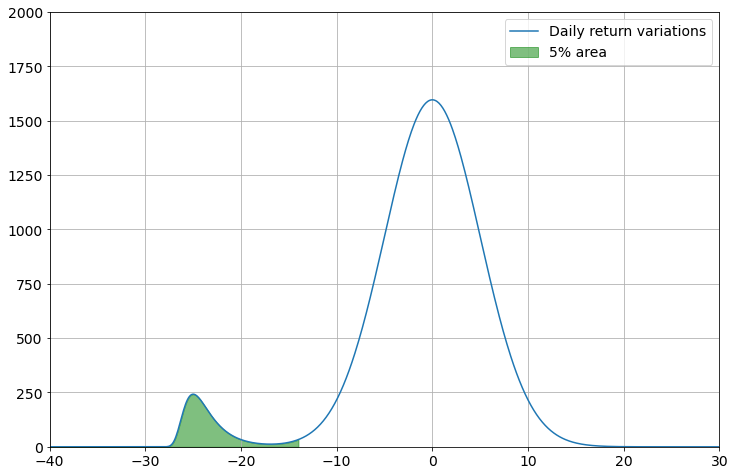
\includegraphics[width=0.8\textwidth]{var}
\end{center}
\makeemptybox{3cm}

\begin{solution}
2 days 95\%-VaR = $14 * \sqrt{2} \approx 19.8$, 1 day 95\%-ES $\approx 23$
\end{solution}

\question The probability of default of two companies can be described by a Poisson process 
\begin{equation*}
P(\lambda, t) = 1 - \exp(-\lambda t)
\end{equation*}
From historical consideration it turns out that $\lambda_A = \lambda_B = 0.05$ (constant over time). 

What is the probability to have both companies defaulted within 1 year from now when the defaults are independent ?
How does this probability change if instead the two marginals are fully correlated ?

\makeemptybox{1.5 cm}

\begin{solution}
%%%% SOLUTION EX 6
\begin{ipython}
import numpy as np

Pd = 1 - np.exp(-0.05*1)
print ("Uncorrelated case: {:.4f}".format(Pd**2))
print ("Fully correlated case: {:.4f}".format(Pd))
\end{ipython}
\begin{ioutput}
Uncorrelated case: 0.024
Fully correlated case: 0.0488
\end{ioutput}
\end{solution}

\end{questions}
\end{document}
